\documentclass[Hovedrapport.tex]{subfiles}
    \begin{document}
%------------------------------------------------------------------------------
%\frontmatter
%\subfile{Rapporten/0000_Forside_appendiks.tex}
%\clearpage                      % T.o.C. begyndes på ny side
%\newpage                        % Resten af siden for T.o.C. tømmes
%\setcounter{page}{0} 	        % Sidetals nr. efter T.o.C
%\mainmatter                     % Lang forklaring...Bare ignorér der!
%---------------------------------------------------
\chapter{Appendiks (Alle)}
    \label{chap:apndx}
        \vspace{-30pt}
        \counterwithout{section}{chapter}
    \renewcommand{\thesection}{A\arabic{section}}

%-------------------------------------------------------------------------------
%--------------------------------- FLASKEDIMENSIONER ---------------------------
%-------------------------------------------------------------------------------        
\section{Flaskedimensioner}
    \label{sec:apndx_flaskedim}        
Det antages at flaskerne er cylinderformede med en højde \SI{15}{cm}, en udvendig diameter på \SI{60}{mm} og en indre diameter på \SI{59,2}{mm}. Højden er oprindelig ikke \SI{15}{cm}, men idet der også skal tages hensyn til at der er en bund på flasken, så bliver der lagt 3 cm til den oprindelig højde som en forsimpling. Den udvendige overfladeareal pr. flaske beregnes da til:
\begin{align}
    A_{u,flaske}=d_u\cdot \pi \cdot h = \SI{285}{cm^2}
\end{align}        
\begin{figure}[H]
    \centering
    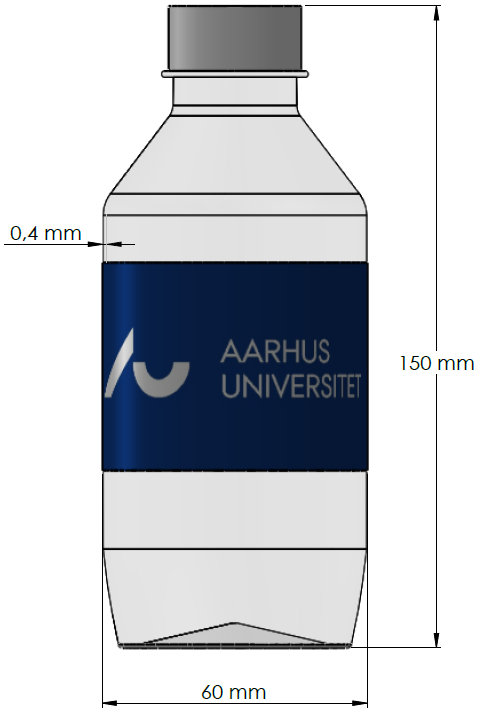
\includegraphics[width=0.5\textwidth]{Billeder/flaskedim.png}
    \caption{\textit{Dimensioner af flasken}}
    \label{fig:apndx_flaskedim}
\end{figure}
\newpage
%-------------------------------------------------------------------------------
%----------------------------- KOMPRESSORBEREGNINGER ---------------------------
%-------------------------------------------------------------------------------
\section{Beregning af kompressorydelsen}
    \label{sec:apndx_kompressorberegninger}
Af figur \ref{fig:apndx_kompressorberegninger1} fremgår beregningerne til bestemmelse af kompressorens sande $h_2$, køletab, tilførte eleffekt samt effektfaktoren for anlægget:
\begin{figure}[H]
    \centering
    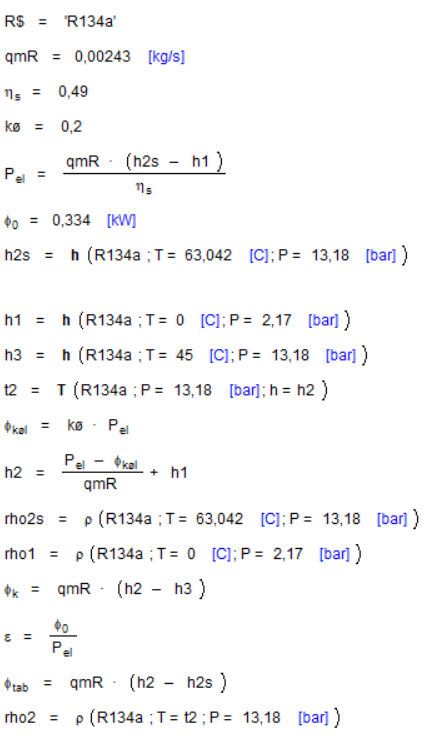
\includegraphics[width=0.45\textwidth]{Billeder/kompressor_bereg1.PNG}
    \caption{\textit{EES udregningerne til beregning af kompressorens kapacitet}}
    \label{fig:apndx_kompressorberegninger1}
\end{figure}

Af figur \ref{fig:apndx_kompressorberegninger2} fremgår resultaterne af beregningen af $h_2$, køletab, tilførte eleffekt samt effektfaktoren:
\begin{figure}[H]
    \centering
    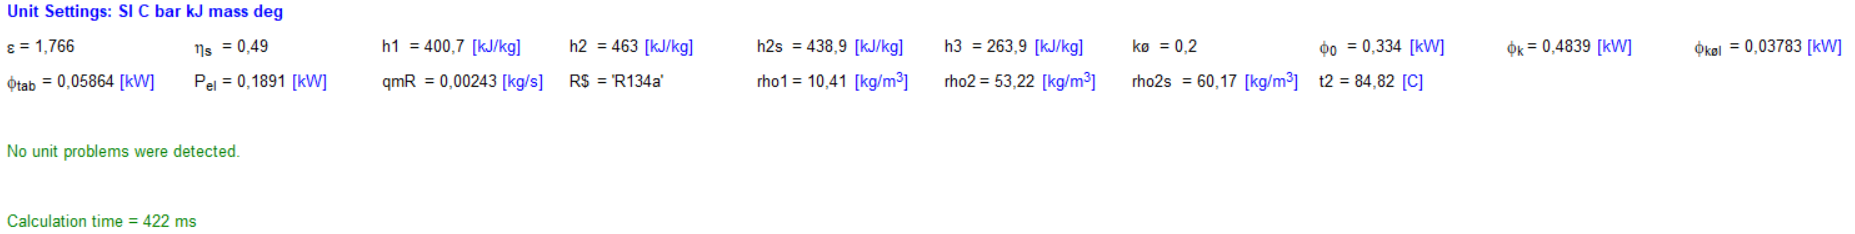
\includegraphics[width=1.0\textwidth]{Billeder/kompressor_bereg2.PNG}
    \caption{\textit{Resultaterne af beregningerne af kompressorydelsen}}
    \label{fig:apndx_kompressorberegninger2}
\end{figure}
\newpage

%-------------------------------------------------------------------------------
%------------------------------ KOMPRESSOR VIRKNINGSGRAD -----------------------
%-------------------------------------------------------------------------------
\section{Beregning af virkningsgrader for kompressor}
    \label{sec:apndx_kompressor_virkningsgrad}
Kompressorens virkningsgrader bestemmes ud fra trykforholdet i systemet. I databladet for kompressoren fremgår testresultater, hvor kompressoren er blevet testet under nogle givne forhold. ved alle testforholdene har kompressoren haft en kondenseringstemperatur på \SI{55}{\celsius}, Hvorefter den er blevet testet ved en varierende fordampningstemperatur. Ved alle fordampningstemperaturer opleves der en overhedning, som vil give en sugegastemperatur på \SI{32}{\celsius}. Entalpierne er aflæst ud fra logp,h-diagrammer fra softwaren \textit{Coolpack} med de givne testforhold, samt en isentropisk virkningsgrad på 1. 
\begin{figure}[H]
    \centering
    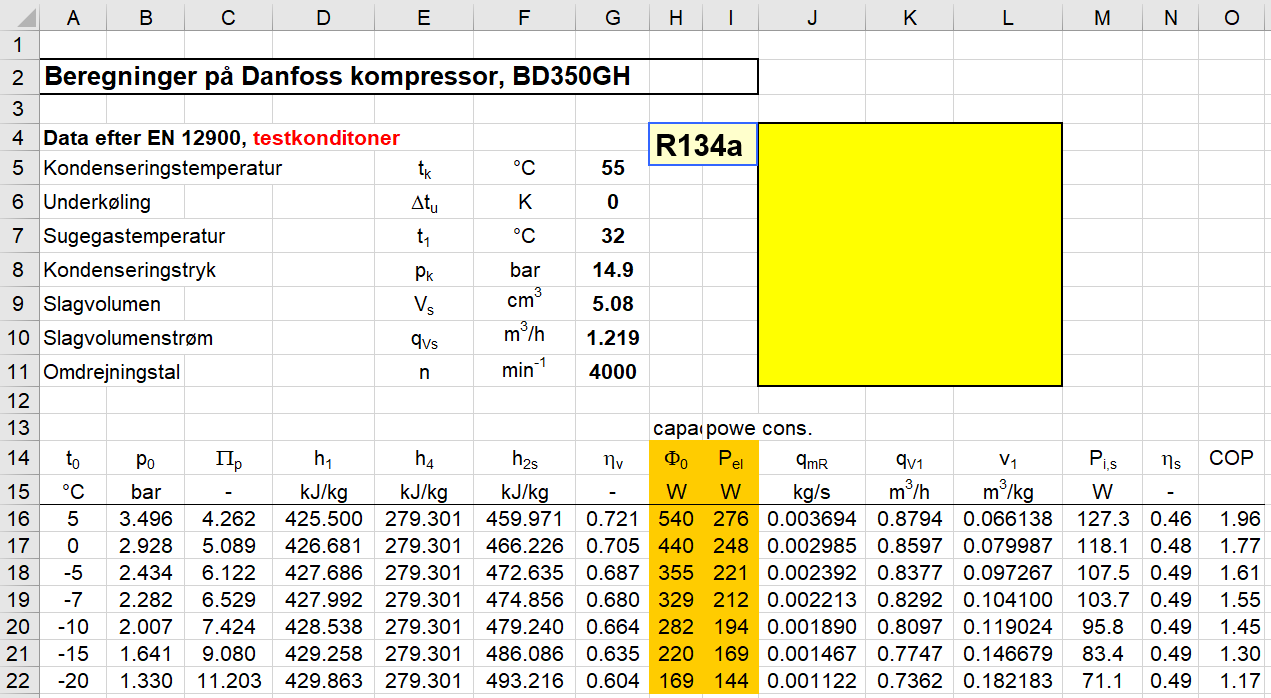
\includegraphics[width=1.0\textwidth]{Billeder/kompressor_excel_1}
    \caption{Oversigt over indtastede og beregnede værdier}
    \label{fig:kompressor_excel_1}
\end{figure}
Nedenfor fremgår formlerne i Excel. værdierne som ønskes beregnet er den isentropiske virkningsgrad, $\eta_s$, den volumetrisk virkningsgrad, $\eta_V$, samt trykforholdet. Disse værdier benyttes til at tegne en graf over virkningsgraderne som funktion af trykforholdet. Denne kan herefter benyttes til at aflæse Virkningsgraderne ud fra det givne trykforhold i systemet.
\begin{figure}[H]
    \centering
    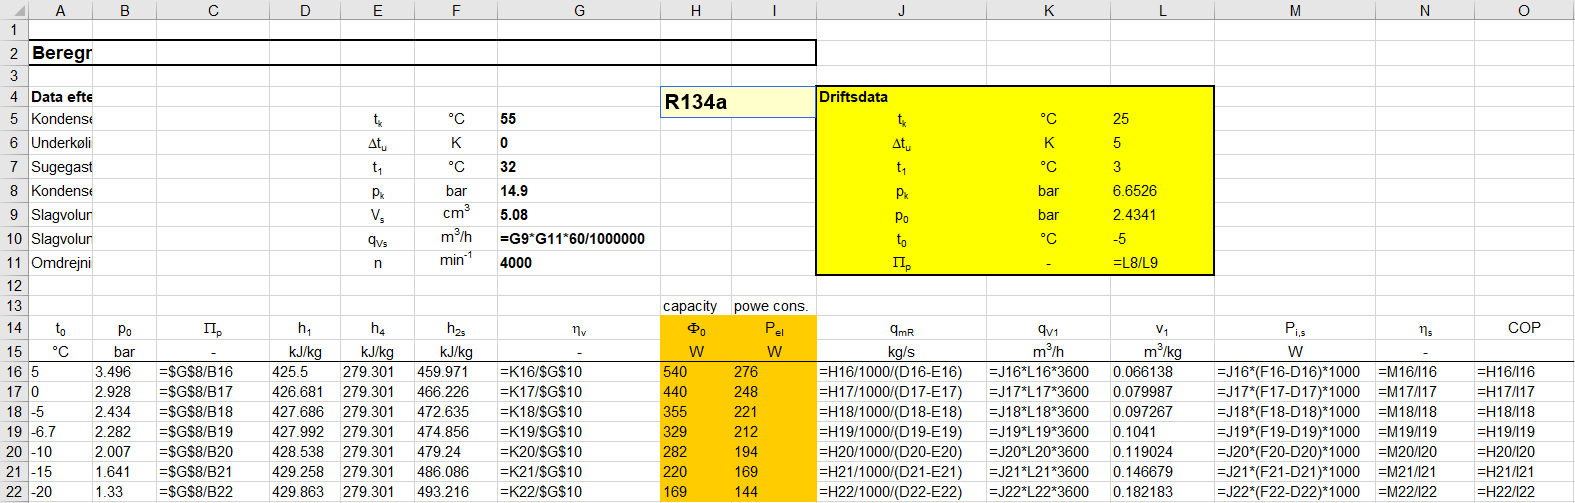
\includegraphics[width=1.0\textwidth]{Billeder/kompressor_excel_4}
    \caption{Formler, som benyttes af excel, til beregning af resterende værdier}
    \label{fig:kompressor_excel_4}
\end{figure}

Den isentropiske og volumetriske virkningsgrad aflæses af figur \ref{fig:kompressor_excel_3}:
\begin{figure}[H]
    \centering
    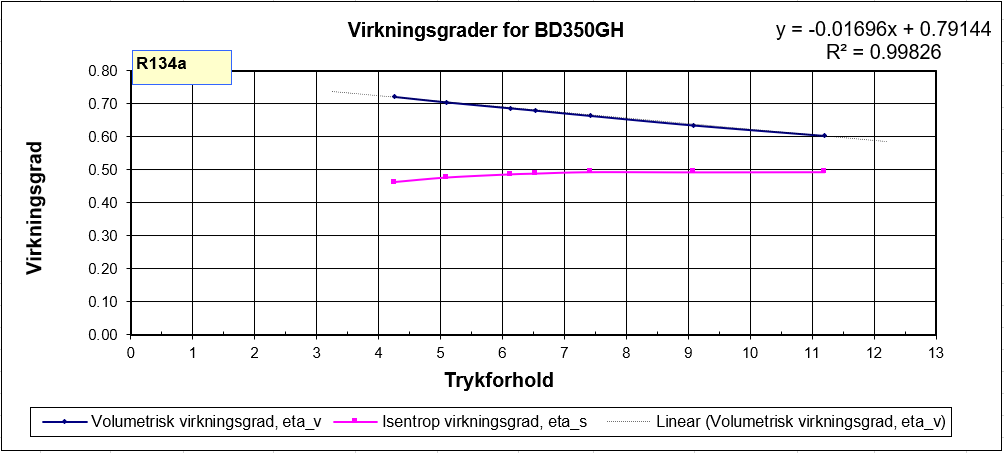
\includegraphics[width=1.0\textwidth]{Billeder/kompressor_excel_3}
    \caption{Graf over virkningsgrader som funktion af trykforhold}
    \label{fig:kompressor_excel_3}
\end{figure}
\newpage

%------------------------------------------------------------------------------
%------------------------ KRAVSPECIFIKATIONER TIL SOFTWARE --------------------
%-------------------------------------------------------------------------------
\section{Kravspecifikationer}
    \label{sec:specs_p24}
Ved udgangen af p2 var der opsat følgende kravspecifikationer for det endelige software, som fremgår af tabel \ref{tab:krav_sam}:
%---------------------------------------------------------------------------------
\begin{table}[H]
	\centering
	\begin{tabular}{|l|l|l|l|} \toprule 
\textbf{Must have}      & \textbf{Should have}          & \textbf{Can have}                     & \textbf{Won't have} \\ \cline{1-4}

Nødstop \cellcolor{green!25}        & Vise enheder\cellcolor{green!25} & Ændring af sprog\cellcolor{red!25}                      & Graf ændrer farve \cellcolor{red!25} \\
PID regulering \cellcolor{green!25} & Brugerskift\cellcolor{green!25}   & Gemme til en SQL-database\cellcolor{red!25}             & Fingertryks login \cellcolor{red!25}     \\
Kalibrering \cellcolor{blue!25}      & Brugerledighed\cellcolor{green!25}                & Tidligere logs\cellcolor{green!25}                        & Kryptering \cellcolor{red!25}            \\
Login funktion \cellcolor{green!25} & Opløsning\cellcolor{orange!25}                     & Maks. tre forsøg \cellcolor{orange!25}                      &       \\
Overskueligt I/F \cellcolor{blue!25}    & Målefejl\cellcolor{blue!25}                      & Nulstil adgangskode \cellcolor{orange!25}                     &                       \\
Datalogning \cellcolor{green!25}         & Måleusikkerheder \cellcolor{blue!25}              & Adgangskodekontrol \cellcolor{green!25}                    &                       \\  
DAQ Kompatibel \cellcolor{blue!25}      & Målefejl\cellcolor{blue!25}                               & Plotte usikkerhed \cellcolor{orange!25}                     &                       \\
Relle data \cellcolor{blue!25}          & \cellcolor{yellow!25} EES Database                              & \cellcolor{green!25} Email adgangskode                                       &                       \\
Sub VI's \cellcolor{green!25}            & \cellcolor{yellow!25}Selvvalgt modstand                              &                                       &                       \\ 
Simulere data \cellcolor{orange!25}      &                               &                                       &                       \\
Brugertype \cellcolor{green!25}         &                               &                                       &   \\
\cellcolor{yellow!25}Opdatering af usikkerheder              &                               &                                       & \\
\cellcolor{yellow!25}Fejlhåndtering                          &                               &                                       & \\
\cellcolor{yellow!25}Kalibrerer individuelle sensorer        &                               &                                       & \\
\cellcolor{yellow!25}Kompressorregulering & & & \\
\cellcolor{yellow!25}Korrigering & & & \\
\cellcolor{yellow!25}Mindst én customized control & & & \\
\bottomrule
	\end{tabular}
	\caption{\textit{Kravene fra udgangen af P2 sorteret efter MoSCoW Metoden}.}
	\label{tab:krav_sam}
	\vspace{-20pt}
\end{table}
%---------------------------------------------------------------------------------
De \emp{\color{green} grønne} felter betegner de krav, som er implementeret forud for leverance P2.2. De \emp{\color{blue} blå} felter betegner de krav, som var ønsket implementeret i P4, ved udgangen af P2, som er lykkes at implementere. De \emp{\color{red} røde} felter betegner de krav, som ikke ønskes implementeret i hverken P2.2 eller P4. De \emp{\color{orange} orange} felter betegner de krav, som var ønsket implementeret i P4, ved udgangen af P2.2, men som er udeladt. Endelig betegner de \emp{\color{yellow} gule} felter kravspecifikationer, som ikke var opsat ved P2.2, men som efterfølgende er identificeret som værende nødvendige for softwarens funktionalitet og derfor implementeret.
\newpage
%------------------------------------------------------------------------------
%------------------------ USIKKERHEDSBUDGET FOR TEMPERATUR --------------------
%-------------------------------------------------------------------------------
\section{Usikkerhedsbudget for type J thermocouples}
    \label{sec:ubudget_temp}
Herunder fremgår usikkerhedsbudgettet for type J thermocouplene, som benyttes i anlægget:
\begin{figure}[H]
	\centering
	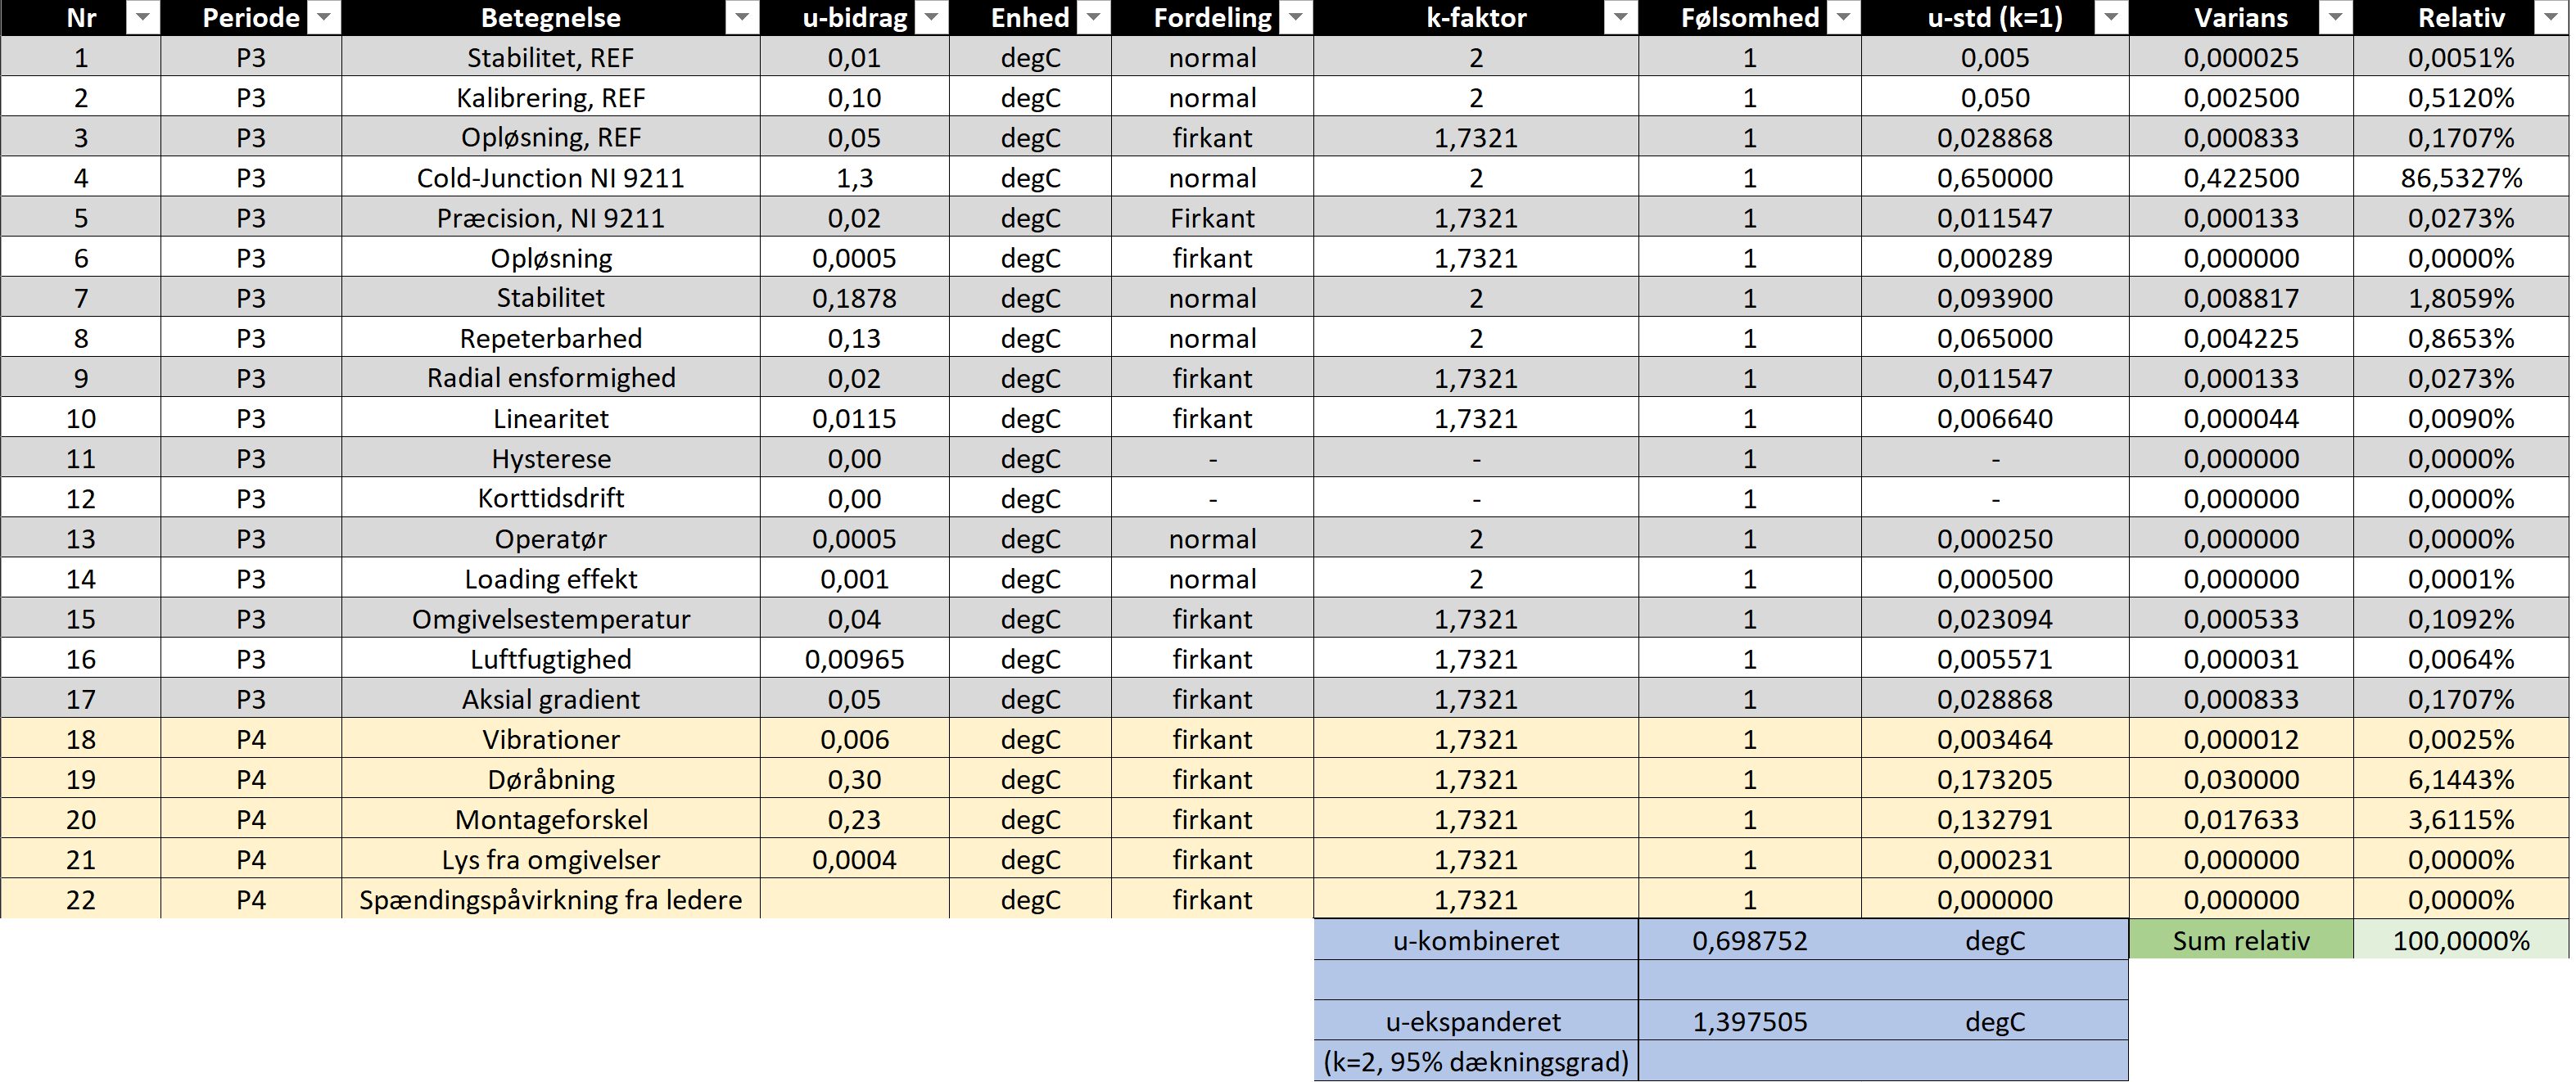
\includegraphics[width=1.0\textwidth]{Billeder/ubudget_temp_endelig.PNG}
	\caption{\textit{Usikkerhedsbudget for thermocouples}.}
	\label{fig:ubudget_temp_endelig}
\end{figure}


%------------------------------------------------------------------------------
%------------------------ USIKKERHEDSBUDGET FOR TRYK --------------------
%-------------------------------------------------------------------------------
\section{Usikkerhedsbudget for AK32 tryktransmittere}
    \label{sec:ubudget_tryk}
Herunder fremgår usikkerhedsbudgettet for \textit{Danfoss AK32} tryktransmittere, som benyttes i anlægget:
\begin{figure}[H]
	\centering
	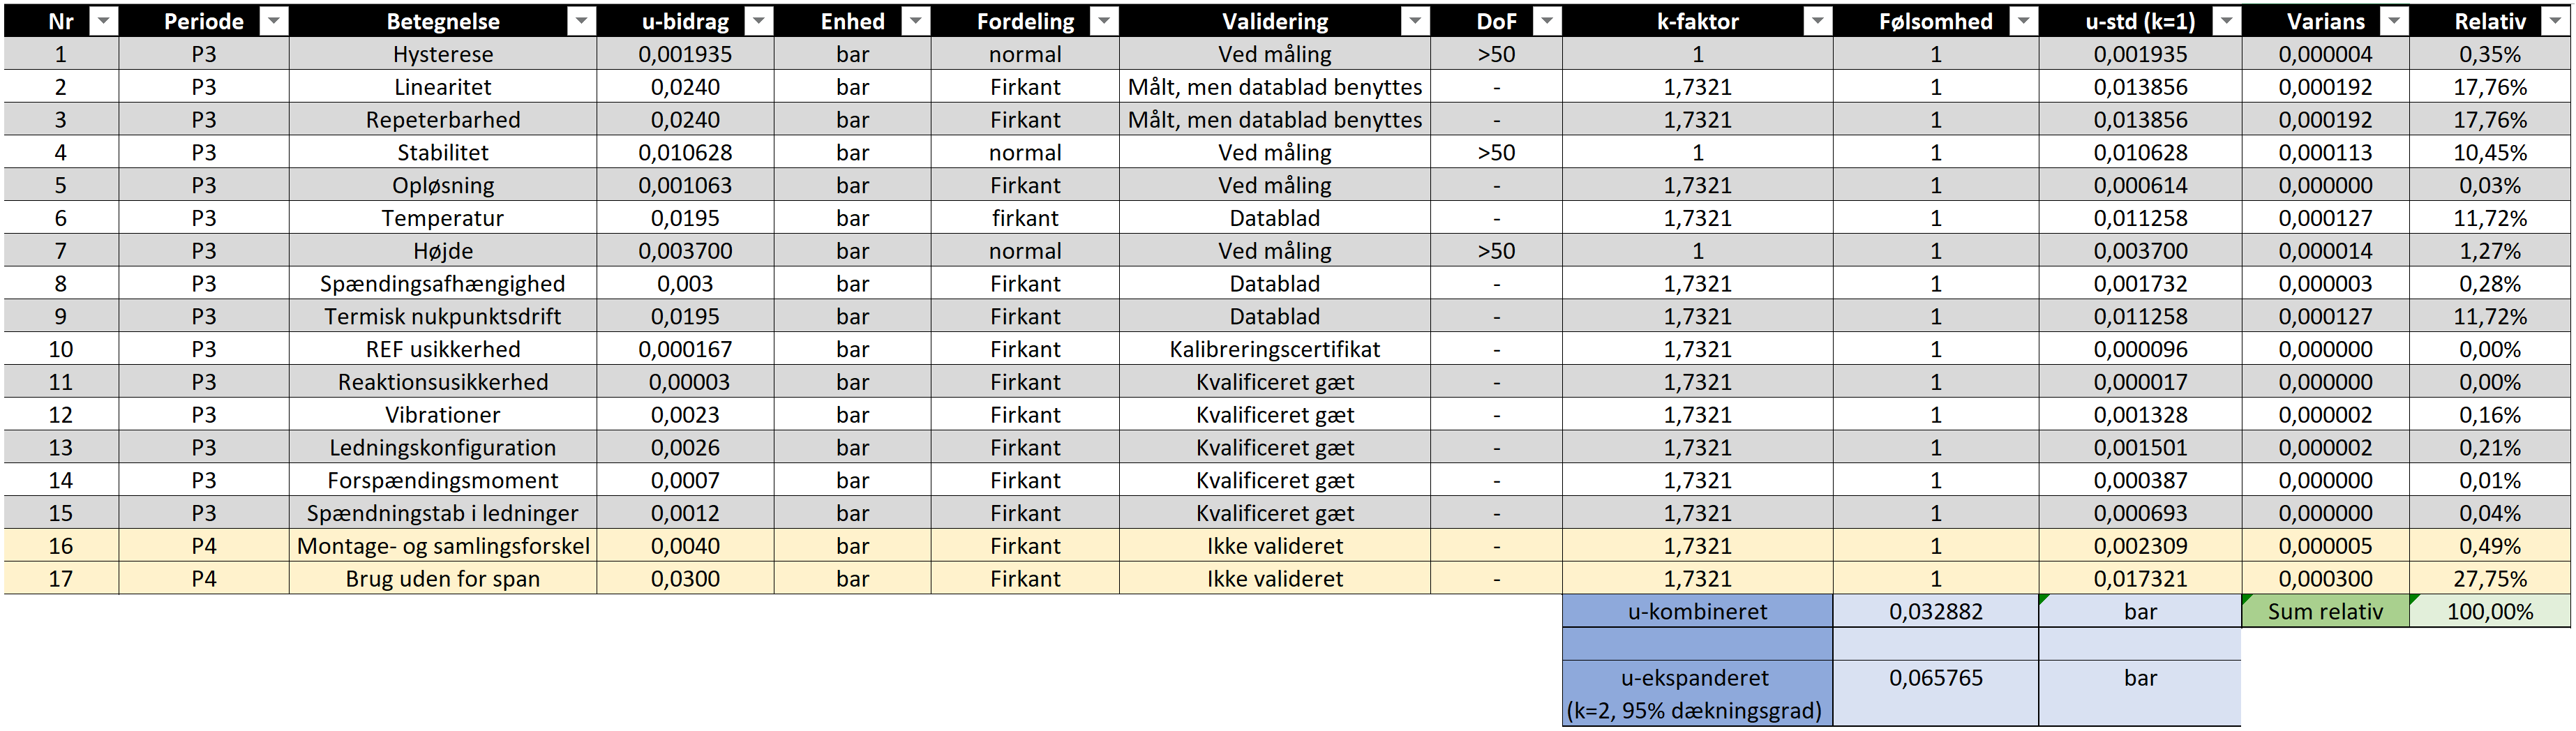
\includegraphics[width=1.0\textwidth]{Billeder/ubudget_tryk_endelig.PNG}
	\caption{\textit{Usikkerhedsbudget for thermocouples}.}
	\label{fig:ubudget_temp_endelig}
\end{figure}
\newpage

%---------------------------------------------------------------------
\section{Varmestrøm ved åbning af dør ved udvendig lufttemperatur på 21 grader}
    \label{sec:doeraabning_21C}
\begin{minipage}{1.0\textwidth}
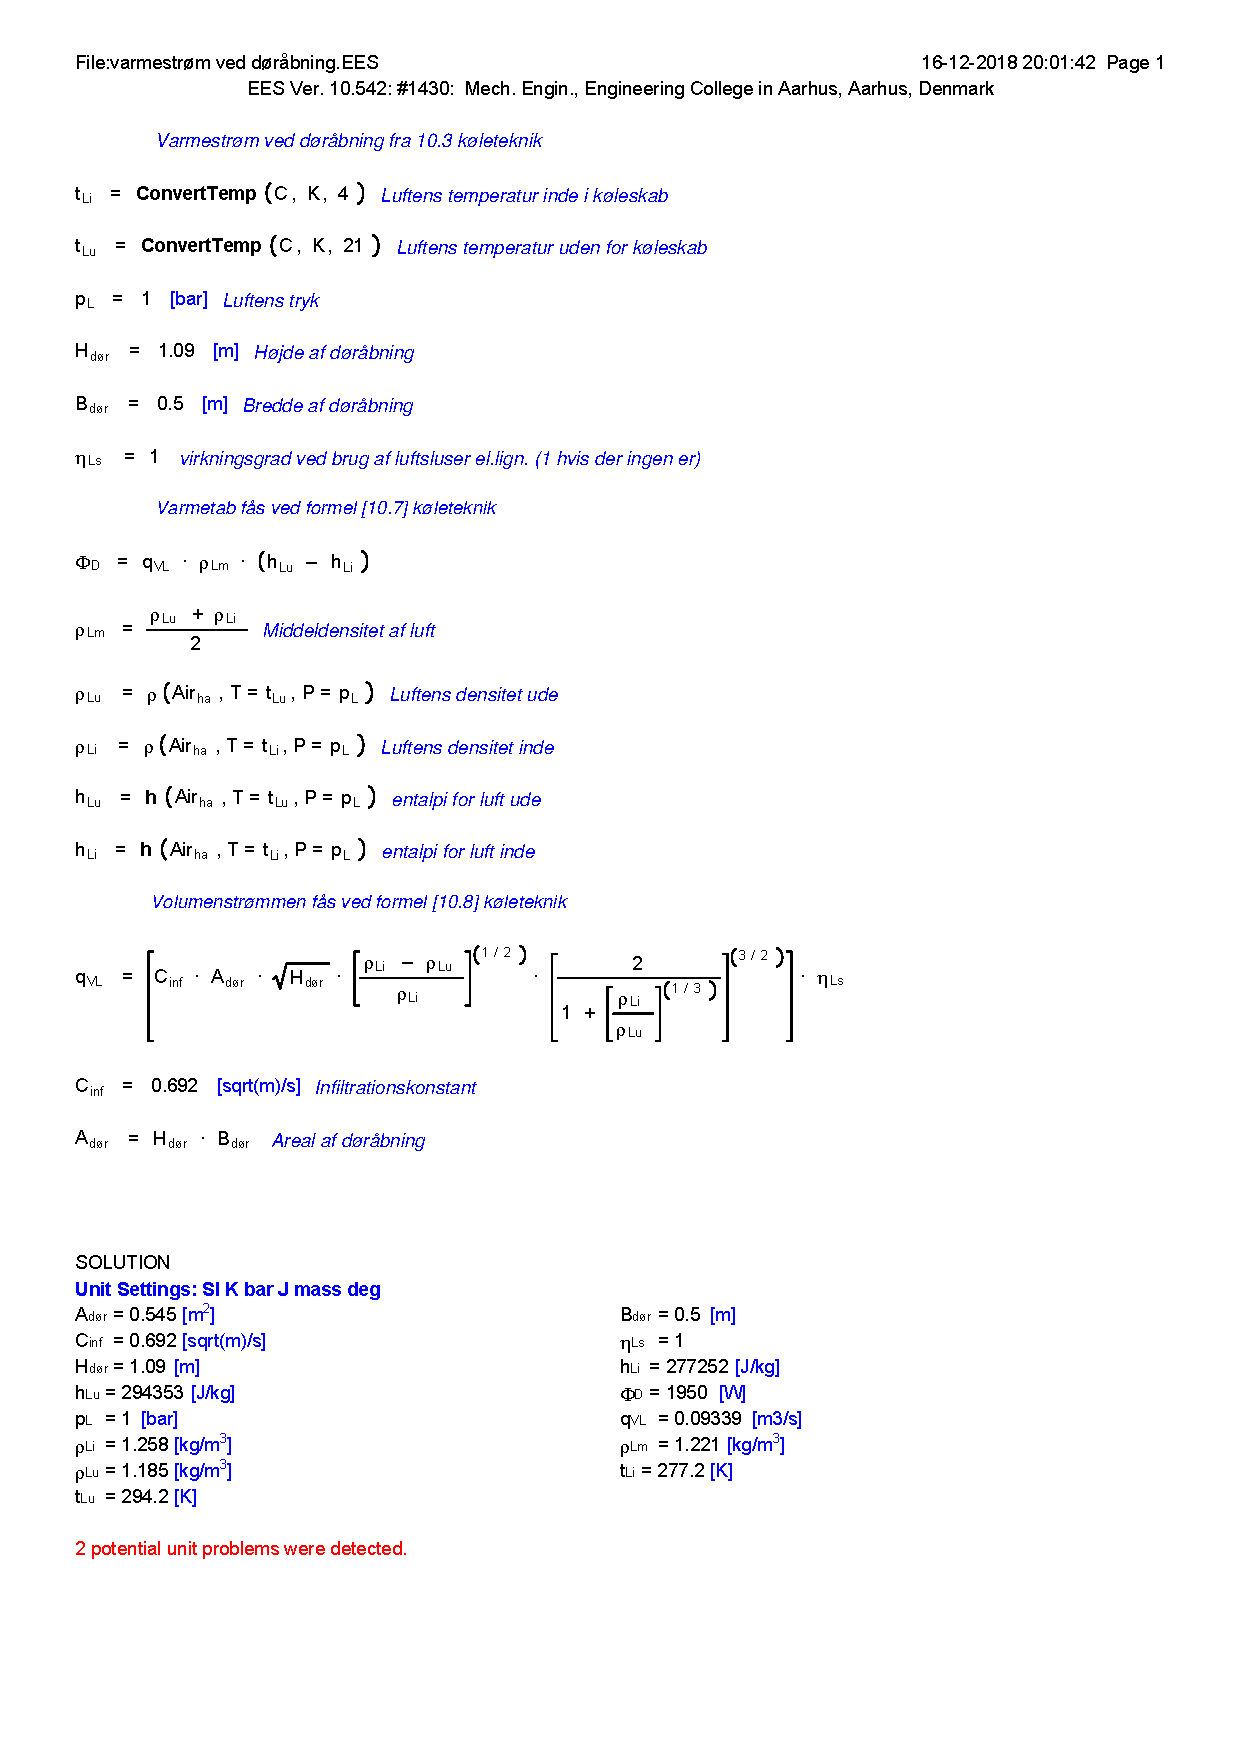
\includepdf[pages={1}, scale=.78, pagecommand={\label{sec:f1t1b}}, offset=0 0cm]{Billeder/dorabning_21C.pdf}
\end{minipage}
\newpage
%----------------------------------------------------------------------------------------------------
%------------------------ Udregning af varmeafgivelse for flasker ved 21 grader --------------------
%---------------------------------------------------------------------------------------------------
\section{Varmeafgivelse for flasker ved 21 grader}
    \label{sec:varmeafgivelse_ved_21grader}

\begin{figure}[H]
	\centering
	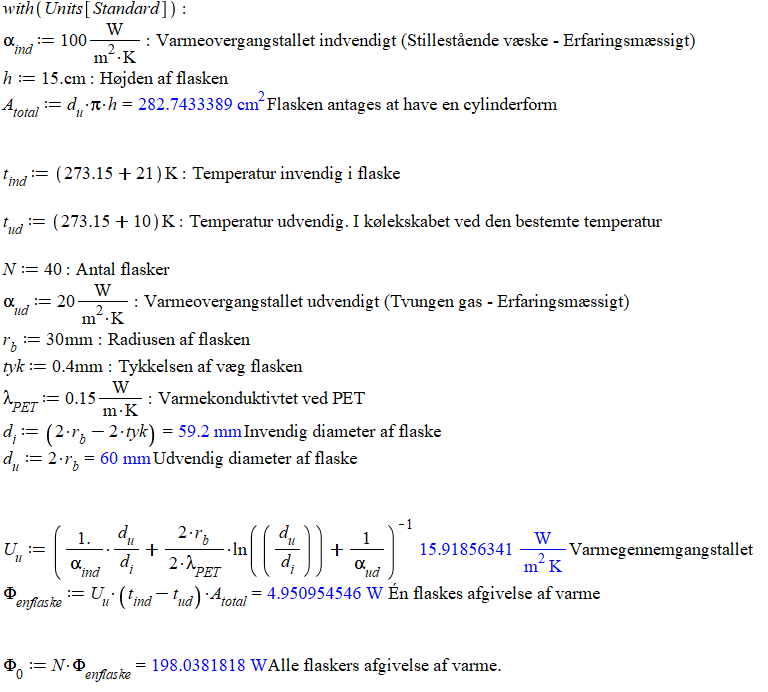
\includegraphics[width=1.0\textwidth]{Billeder/varme_ved_21grader.PNG}
	\caption{\textit{Varmeafgivelse for flasker ved 21 grader}.}
	%\label{fig:ubudget_temp_endelig}
\end{figure}
\newpage
%---------------------------------------------------------------------------------------------------
%------------- Udregning af varmestrøm ved døråbning ved lufttemperatur på 21 grader ---------------
%---------------------------------------------------------------------------------------------------



%-------------------------------------------------------------------------------
%---------------------------------- PROCESEVALUERING ---------------------------
%-------------------------------------------------------------------------------
\newpage
\section{Procesbeskrivelse}
%-------------------------------------------------------------------------------
Der er igennem projektet gjort nogle erfaringer. Disse erfaringer er blevet diskuteret blandt gruppens medlemmer, og der er bred enighed fra alle disse omkring det, der bliver beskrevet i følgende afsnit. Procesbeskrivelsen opdeles i to sektioner; 'Faglige erfaringer' og 'samarbejdets erfaringer'.

\textbf{Faglige erfaringer:} \\
Inden projektets begyndelse var det gruppens forventning at få en dybere forståelse for, hvordan et kølesystem fungerer samt hvordan der regnes på diverse elementer heraf. Dette er også vurderet til at være indfriet, da der igennem forløbet har været et stort fokus på at udføre udregninger på bl.a. fordamperen og kondensatoren.   
Alle gruppemedlemmer føler, at de har fået en dybere forståelse for, hvordan et køleteknisk system fungerer samt hvordan de individuelle dele influerer kredsprocessen. 

Afslutningsvis har gruppen også erfaret vigtigheden af gode illustrationer til at hjælpe formidlingen af komplekse forklaringer. 

\textbf{Samarbejdets erfaringer:} \\
I starten af projektet er der udarbejdet en tidsplan. Denne tidsplan blev inddraget i flere sammenhænge i starten af projektet. Dette betyder, at der i denne perode var et godt overblik over projektet. Gruppens medlemmer mistede dog fokus på tidsplanen og sidste måned af projektet blev denne overhovedet ikke benyttet, idet nye deadlines blev aktuelle. Gruppen blev her en smule opdelt iform af deadlines i Instrumenteringsfaget. 
Hele denne oplevelse har været med til at cementere vigtigheden af at bevare overblikket, og dertil er en tidsplan et uvurderlig værktøj.

Igennem projektet har det virket godt at have mindre løbende deadlines. Dette har været iform af bl.a. milepæl 1 og 2, de 4 portifolioopgaver samt mindre deadlines selv opstillet af gruppen. De løbende deadlines har gjort at gruppen har arbejdet effektivt og målrettet for at opnå kravene til fjerde semester.

Overordnet er samarbejdet i gruppen forløbet relativt problemfrit. Dette hænger sandsynligtvis også sammen med at gruppen arbejdede sammen i det foregående semester. Derfor kender de forskellige medlemmer hinandens styrker og svagheder, hvilket har været med til at højne effektiviteten.

Alt i alt er alle medlemmer tilfredse med forløbet, og der vurderes et stort udbytte, både fagligt og personligt. Dette semesterprojekt har givet gruppens medlemmer et indblik, hvordan fremtidig projektarbejde kan forløbe på en tilfredsstillende måde. 
    \newpage

%-------------------------------------------------------------------------------
%---------------------------------- TIDSPLAN FOR PROJEKT -----------------------
%-------------------------------------------------------------------------------
\section{Tidsplaner}
\begin{figure}[H]
    \centering
    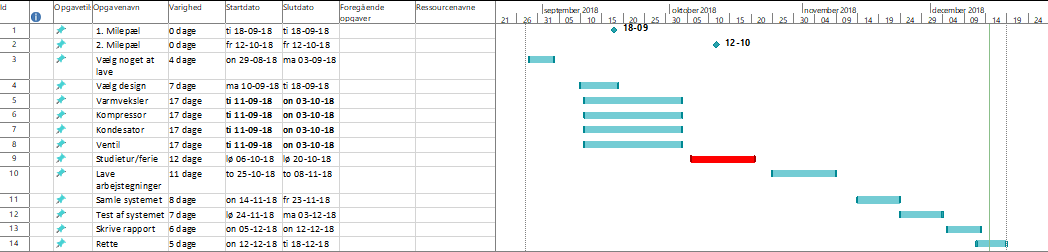
\includegraphics[width=\textwidth]{Billeder/opr_time.png}
    \caption{Oprindelig tidsplan}
    \label{fig:opr_time}
\end{figure}

\begin{figure}[H]
    \centering
    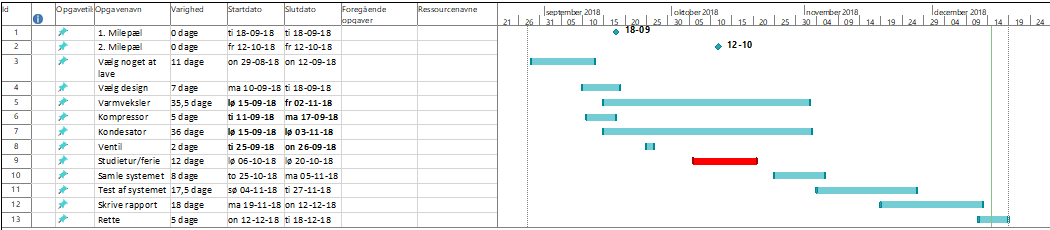
\includegraphics[width=\textwidth]{Billeder/end_time.png}
    \caption{Endelig tidsplan}
    \label{fig:end_time}
\end{figure}


%%%%%%%%%%%%%%% EES makro %%%%%%%%%
\section{EES makro}
\label{sec:apndx_EES_makro}
Nedenstående ses den EES makro 
\begin{figure}[H]
    \centering
    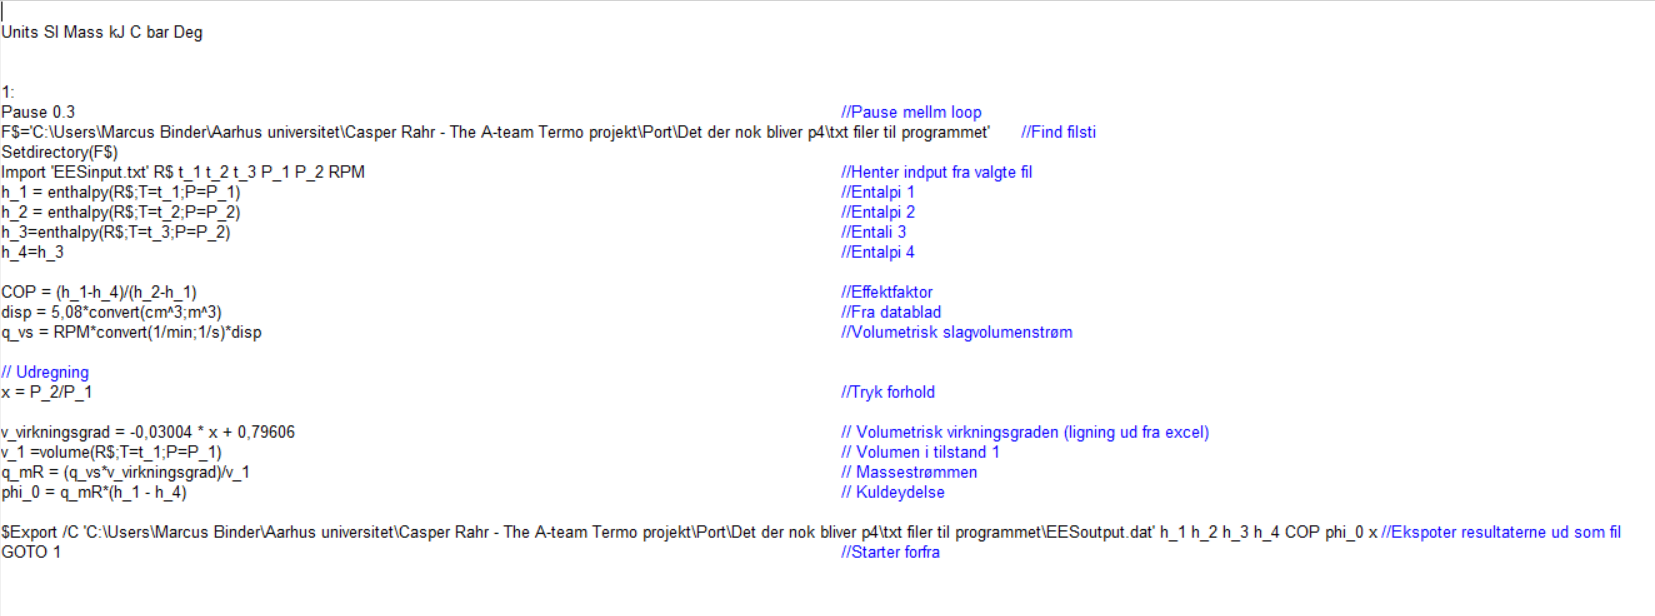
\includegraphics[width=\textwidth]{Billeder/EES_makro.png}
    \caption{Oprindelig tidsplan}
    \label{fig:apndx_EES_makro}
\end{figure}
\newpage

%%%%%%%%%%%%%%%- forsøg 1 test 1 a
\section{Forsøg 1 test 1 a}
\label{sec:f1t1a}
I nedenstående beregninger vil den maksimale kuldeydelse, $\Phi_{max}$, blive beregnet for situationen, hvor køleskabsdøren er helt åben i Forsøg 1, test 1. Desuden vil overhedningen også blive bestemt samt de tilhørende usikkerheder for resultaterne. Som i de efterfølgende appendikser vil der følge en kort konklusion over resultaterne efter appendikset. 
\begin{minipage}{1.0\textwidth}
\includepdf[pages={1}, scale=.7,  pagecommand={\pagestyle{fancy}}, offset=0 0cm]{Billeder/forsøg1_test1_a.pdf}
\end{minipage}

\includepdf[pages={2,3}, scale=.8,pagecommand={\pagestyle{fancy}}, offset=0 0cm]{Billeder/forsøg1_test1_a.pdf} 

Forsøg 1, test 1 b: Således er den maksimale kuldeydelse bestemt til \SI{612,8}{W} og \SI{565,8}{W} ud fra henholdsvis kølemiddel og luft. Overhedningen er fundet til \SI{7,9}{K}

%%%%%%%%%%%%%%%- forsøg 1 test 1 b
\newpage
\section{Forsøg 1 test 1 b}

Udregninger nedenfor i \textit{EES } svarer til de i forsøg 1 test 1a. $\Phi_{max}$ vil blive beregnet sammen med overhedningen og usikkerhederne 

\begin{minipage}{1.0\textwidth}
\includepdf[pages={1}, scale=.6, pagecommand={\label{sec:f1t1b}}, offset=0 0cm]{Billeder/forsøg1_test1_b.pdf}
\end{minipage}

\includepdf[pages={2,3}, scale=.8,pagecommand={\pagestyle{fancy}}, offset=0 0cm]{Billeder/forsøg1_test1_b.pdf}

Forsøg 1, test 1 b: Dermed er den maksimale kuldeydelse lig med \SI{623,5}{W} og \SI{603,7}{W} beregnet ved henholdsvis kølemiddel og luft. Overhedningen er bestemt til \SI{7,8}{K}.
%%%%%%%%%%%%%%%- forsøg 1 test 2
\newpage
\section{Forsøg 1 test 2}
\label{f1t2}
Nedenstående beregninger i \textit{EES} tager afsæt i scenariet, hvor temperaturen inde i køleskabet er \SI{10}{\celsius} under nedkølingen. Kuldeydelsen vil hertil blive bestemt. 

\begin{minipage}{1.0\textwidth}
\includepdf[pages={1}, scale=.7, pagecommand={\pagestyle{fancy}}, offset=0 0cm]{Billeder/forsøg1_test2.pdf}
\end{minipage}

\includepdf[pages={2,3}, scale=.8,pagecommand={\pagestyle{fancy}}, offset=0 0cm]{Billeder/forsøg1_test2.pdf}

Således er kuldeydelsen blevet bestemt til \SI{510,4}{W} via kølemidlet i forsøg 1 test 2. Kuldeydelsen bestemt via luften er beregnet til \SI{421}{W}.

%%%%%%%%%%%%%%%- forsøg 1 test 3 a
\newpage
\section{Forsøg 1 test 3 a}
\label{sec:bil_tryk}
I forsøg 1 test 3 a bestemmes kuldeydelsen ved stationær tilstand og en temperatur på \SI{4}{\celsius}. Dette gøres via \textit{EES}.

\begin{minipage}{1.0\textwidth}
\includepdf[pages={1}, scale=.7, pagecommand={\pagestyle{fancy}}, offset=0 0cm]{Billeder/forsøg1_test3_a.pdf}
\end{minipage}

\includepdf[pages={2,3}, scale=.8,pagecommand={\pagestyle{fancy}}, offset=0 0cm]{Billeder/forsøg1_test3_a.pdf}

Således er kuldeydelsen via luft og kølemiddel bestemt til henholdsvis \SI{431,5}{W} og \SI{406,2}{W} i forsøg 1 test 3 a.

%%%%%%%%%%%%%%%- forsøg 1 test 3 b
\newpage
\section{Forsøg 1 test 3 b}
\label{sec:f1t3b}

Via \textit{EES} bestemmes kuldeydelsen for situationen, hvor køleskabet befinder sig i en stationær tilstand og har en temperatur på \SI{4}{\celsius}

\begin{minipage}{1.0\textwidth}
\includepdf[pages={1}, scale=.7, pagecommand={\pagestyle{fancy}}, offset=0 0cm]{Billeder/forsøg1_test3_b.pdf}
\end{minipage}

\includepdf[pages={2,3}, scale=.8,pagecommand={\pagestyle{fancy}}, offset=0 0cm]{Billeder/forsøg1_test3_b.pdf}

I forsøg 1 test 3b er kuldeydelsen blevet beregnet til \SI{335,3}{W} på baggrund af kølemidlet, mens den på baggrund af luften er bestemt til \SI{293,2}{W}.
%%%%%%%%%%%%%%%- forsøg 3 
\newpage
\section{Forsøg 3 }  
\label{sec:f3}
    
Den teoretiske værdi for varmestrømmen, som tilføres ved åbning af køleskabsdøren ønskes beregnet via \textit{EES}. Det bør her bemærkes, at de angivne \textit{unit problems} er knyttet til infiltrationskonstanten, hvor \textit{EES} ikke kender den angivne enhed. 

\begin{minipage}{1.0\textwidth}
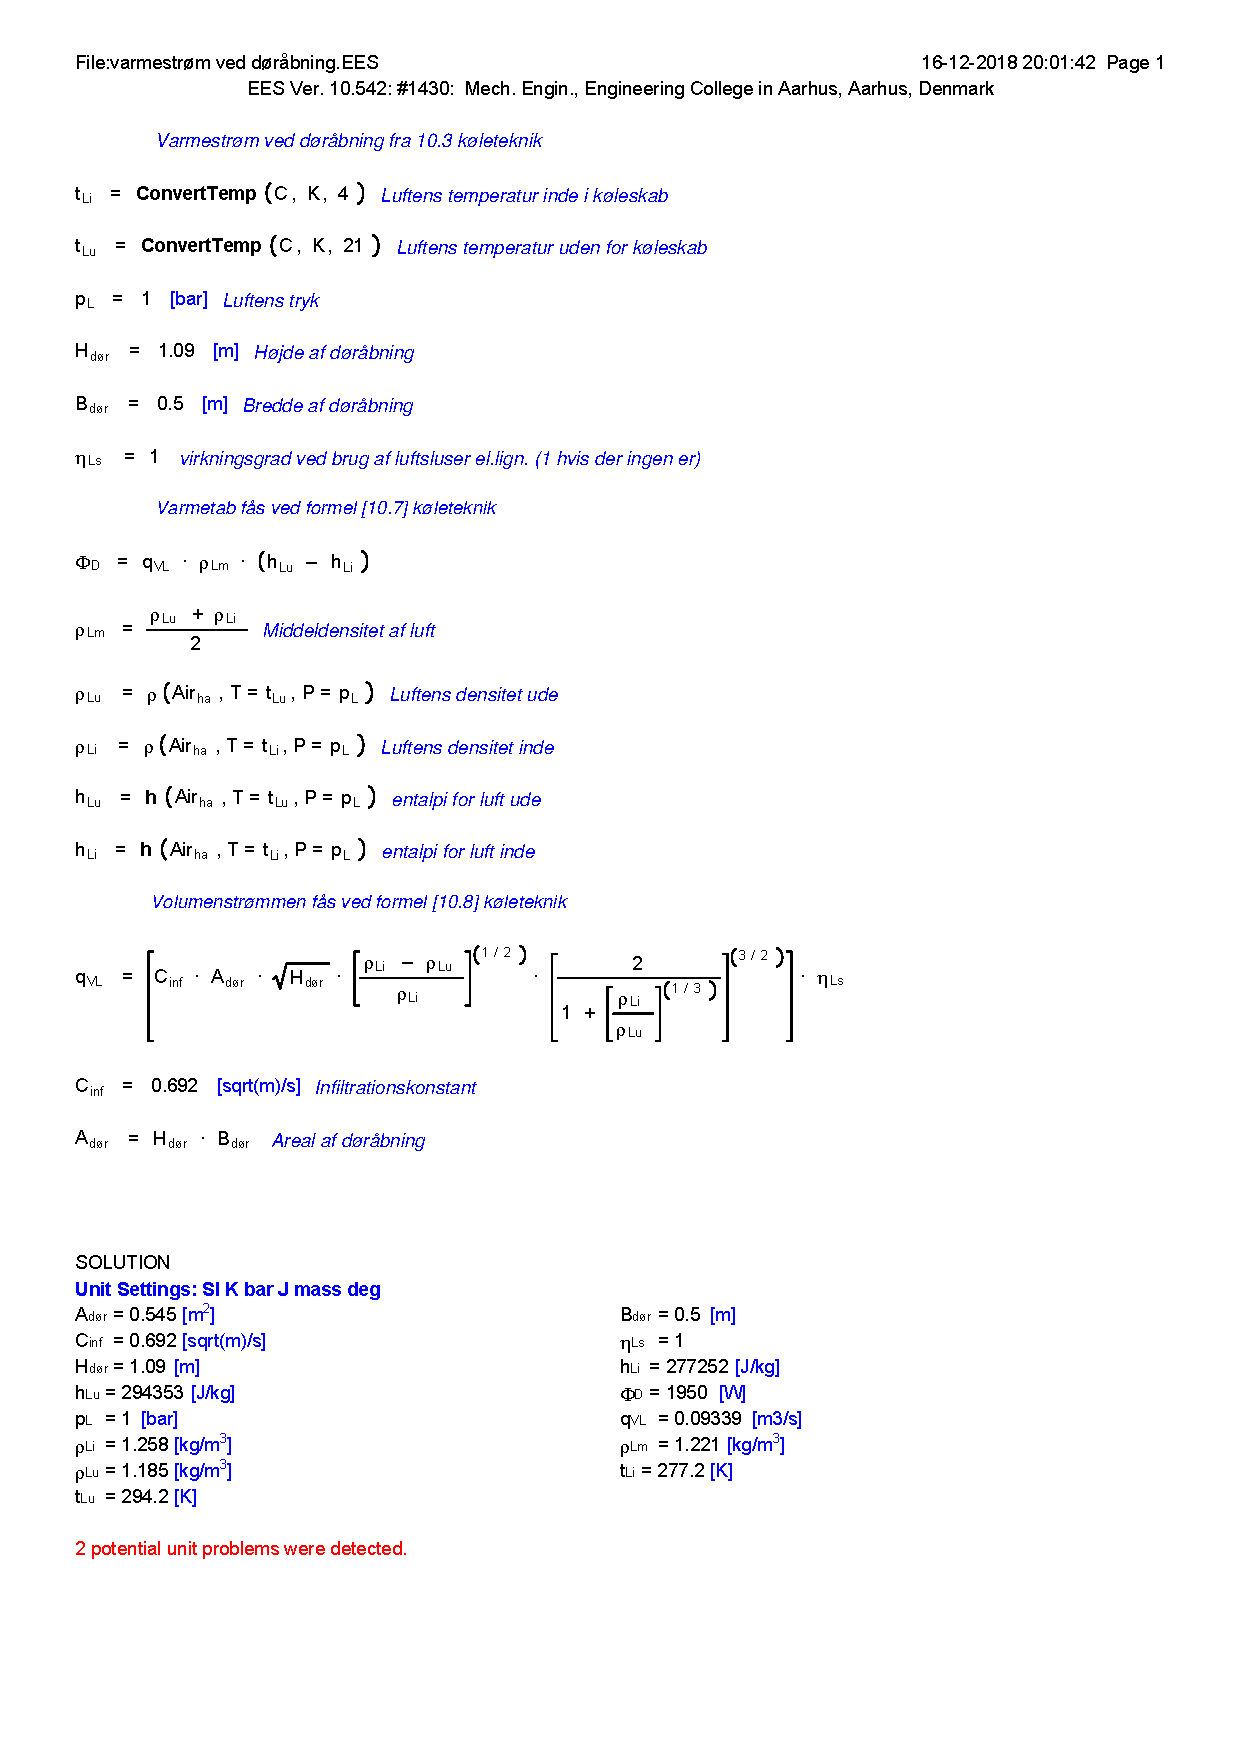
\includepdf[pages={1}, scale=.7, pagecommand={\pagestyle{fancy}}, offset=0 0cm]{Billeder/dorabning_21C.pdf}
\end{minipage}

\newpage
Således er den teoretiske værdi for den tilførte varmestrøm ved åbning af døren bestemt til \SI{1950}{W}.
%%%%%%%%%%%%%%%- forsøg 4 
\newpage
\newpage
\section{Forsøg 4}
Under forsøg 4 er 40 flasker vand blevet indsat i køleskabet, for at blive kølet ned fra stuetemperatur. Det ønskes at bestemme en funktionsligning, som beskriver flaskernes nedkølingsforløb. Dette gøres via softwaren \textit{Logger Pro}. Temperaturforløbene med dertilhørende regressioner fremgår af nedenstående figurer:

\begin{figure}[H]
    \centering
    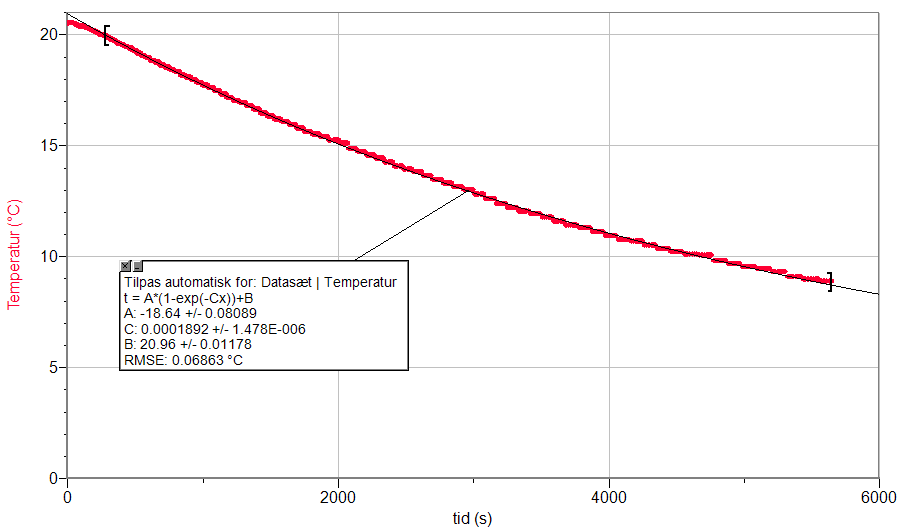
\includegraphics[width=\textwidth]{Billeder/tempreg1}
    \caption{Resultat af regression på temperaturforløb for Flaske 1}
    \label{fig:tempreg1}
\end{figure}

\begin{figure}[H]
    \centering
    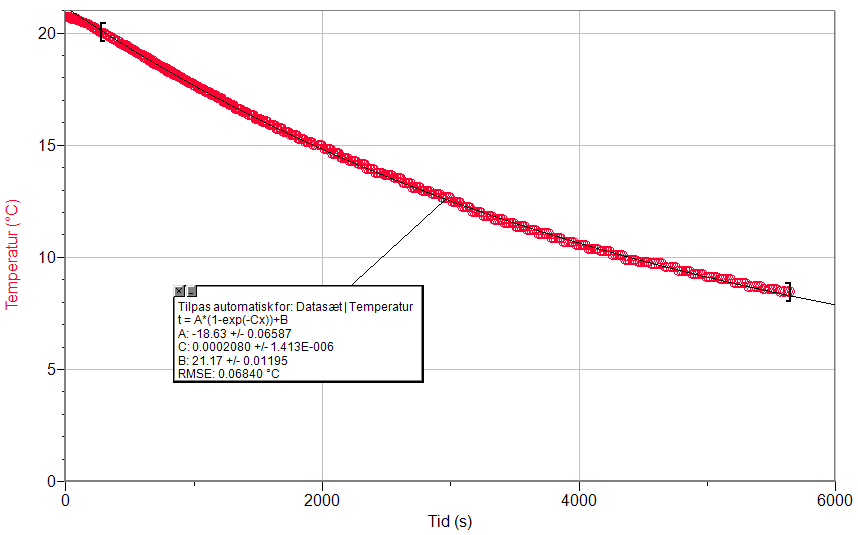
\includegraphics[width=\textwidth]{Billeder/tempreg2}
    \caption{Resultat af regression på temperaturforløb for Flaske 2}
    \label{fig:tempreg2}
\end{figure}

\begin{figure}[H]
    \centering
    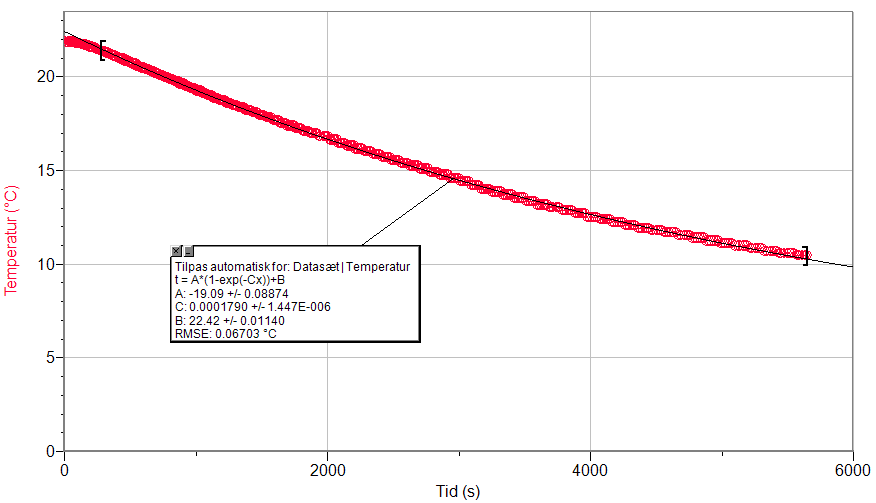
\includegraphics[width=\textwidth]{Billeder/tempreg3}
    \caption{Resultat af regression på temperaturforløb for Flaske 3}
    \label{fig:tempreg3}
\end{figure}

Dernæst ønskes det at bestemme temperaturforløbenes maksimale hældning, i det område, regressionen spænder over. Dette gøres i maple, som fremgår nedenfor.

\begin{minipage}{1.0\textwidth}
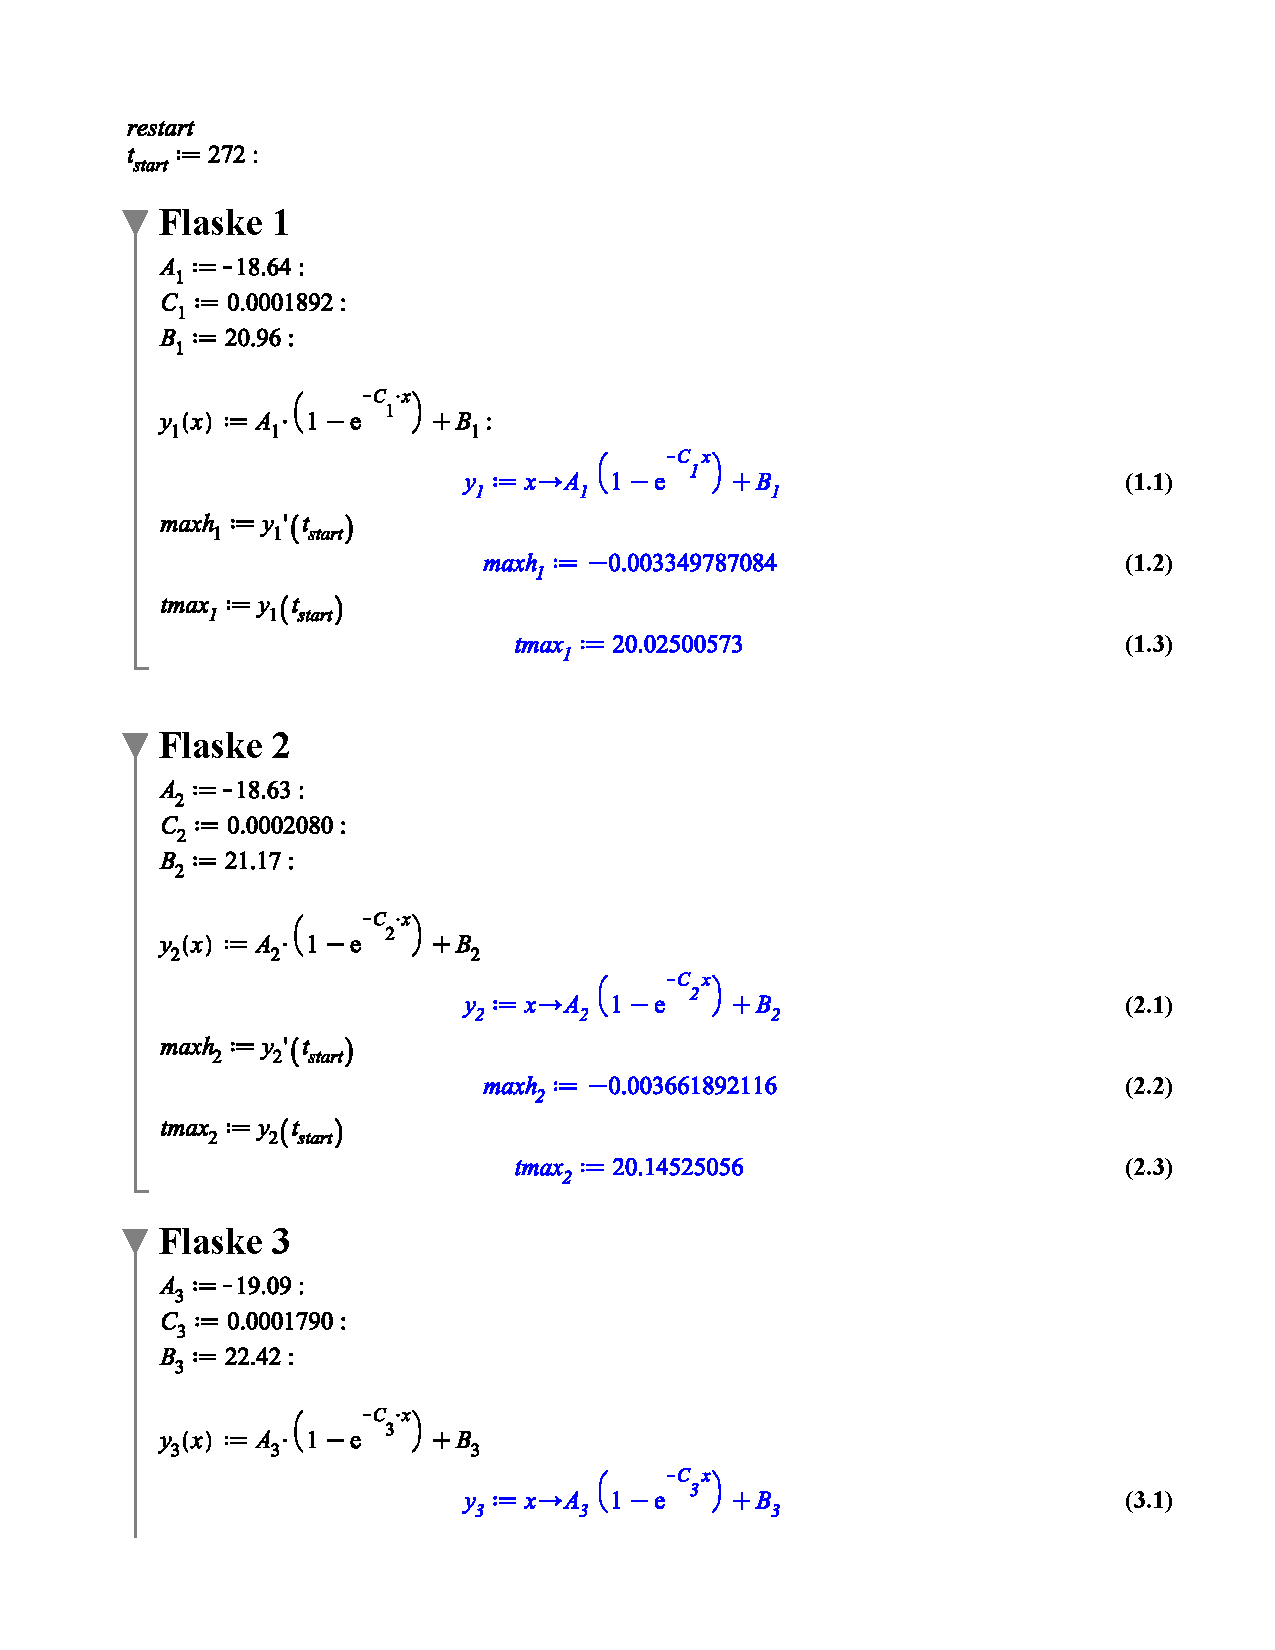
\includepdf[pages={1}, scale=.8, pagecommand={\label{sec:flaskehaeldning}}, offset=0 0cm]{Billeder/flaskehaeldning_maple.pdf}
\end{minipage}


\includepdf[pages={2}, scale=.8,pagecommand={\pagestyle{fancy}}, offset=0 0cm]{Billeder/flaskehaeldning_maple.pdf}

Ud fra de fundne værdier for hældning og temperatur, ved samme punkt, vil varmestrømmet fra flaskerne blive beregnet i \textit{EES} efter nedenstående fremgangsmåde:
\begin{minipage}{1.0\textwidth}
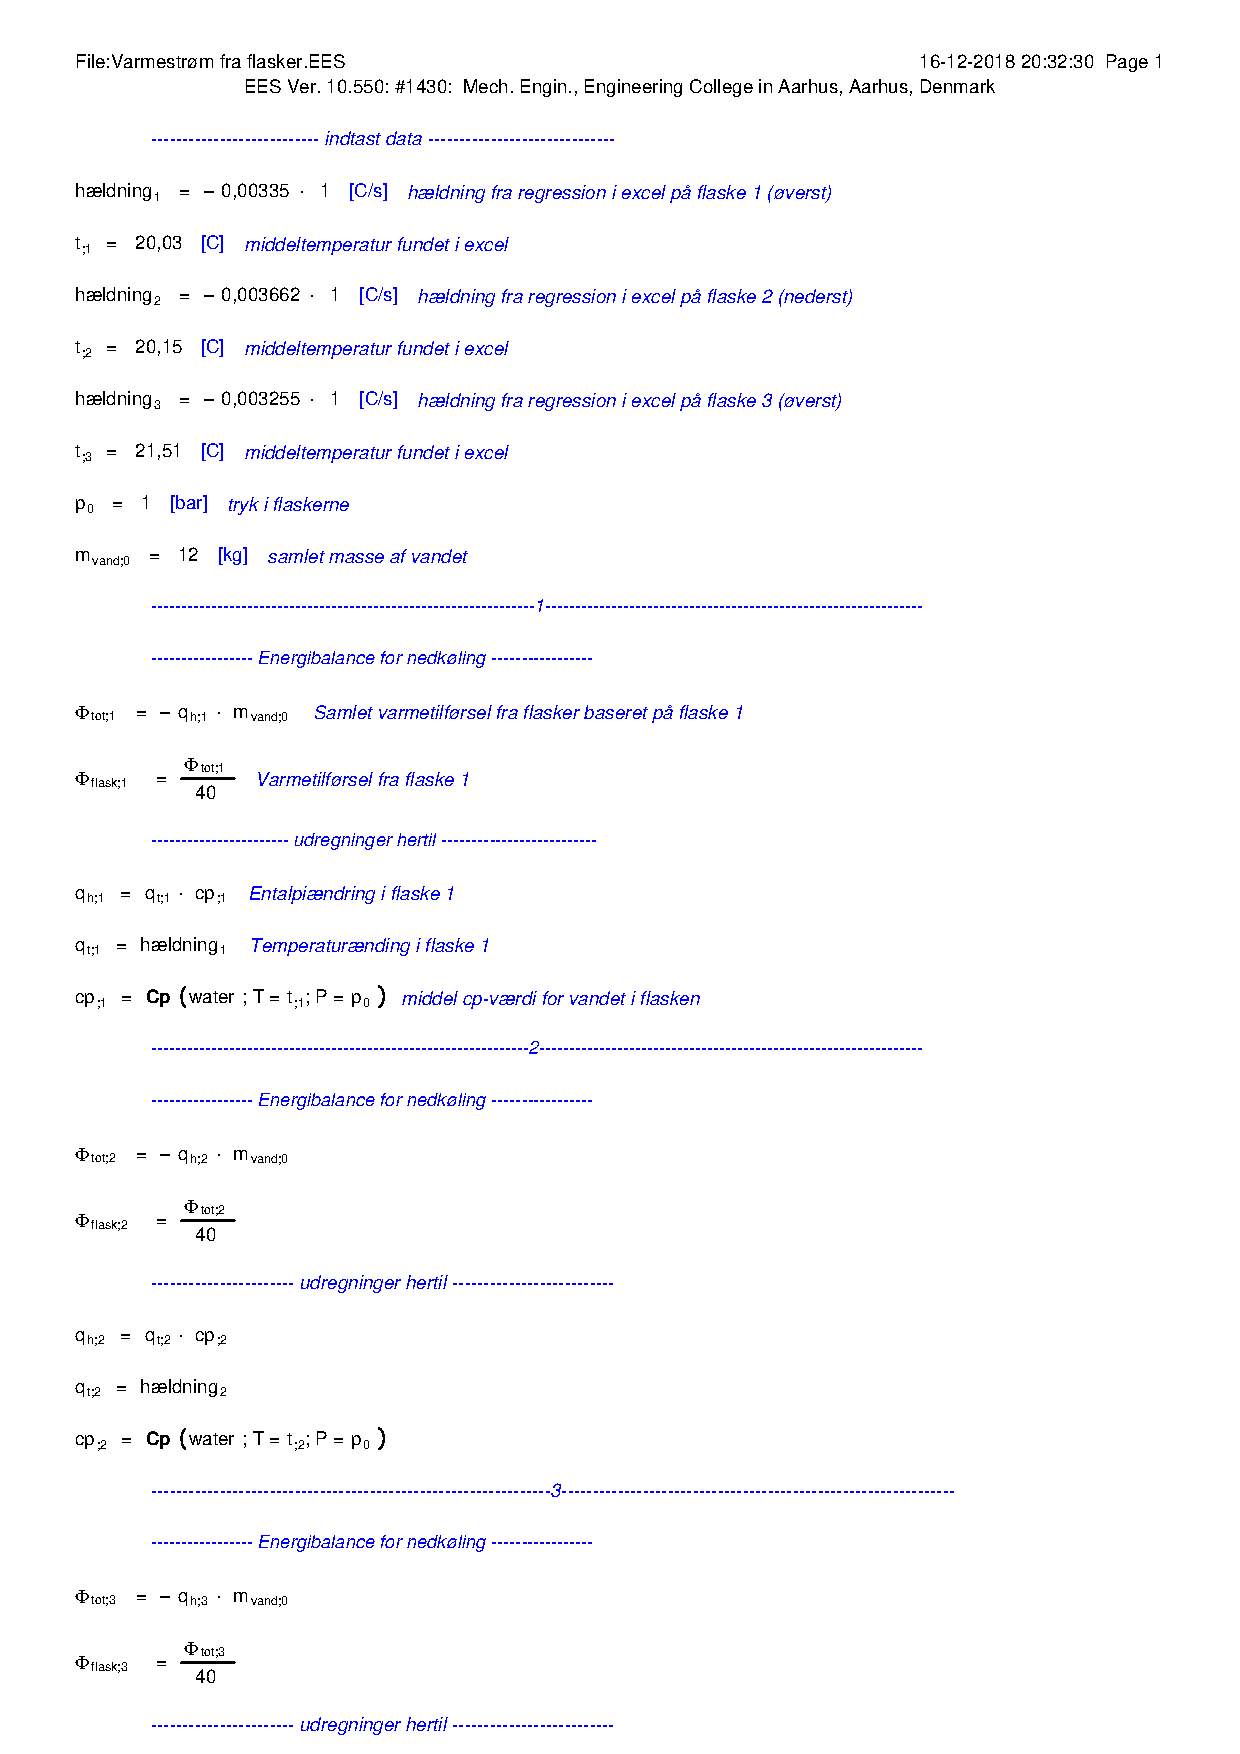
\includepdf[pages={1}, scale=.8, pagecommand={\label{sec:f4}}, offset=0 0cm]{Billeder/forsøg4.pdf}
\end{minipage}


\includepdf[pages={2}, scale=.8,pagecommand={\pagestyle{fancy}}, offset=0 0cm]{Billeder/forsøg4.pdf}

% -----------------proto billeder-------------------
\newpage

\section{Bud på viderebygget prototype}
\label{sec:proto1}
\begin{figure}[H]
    \centering
    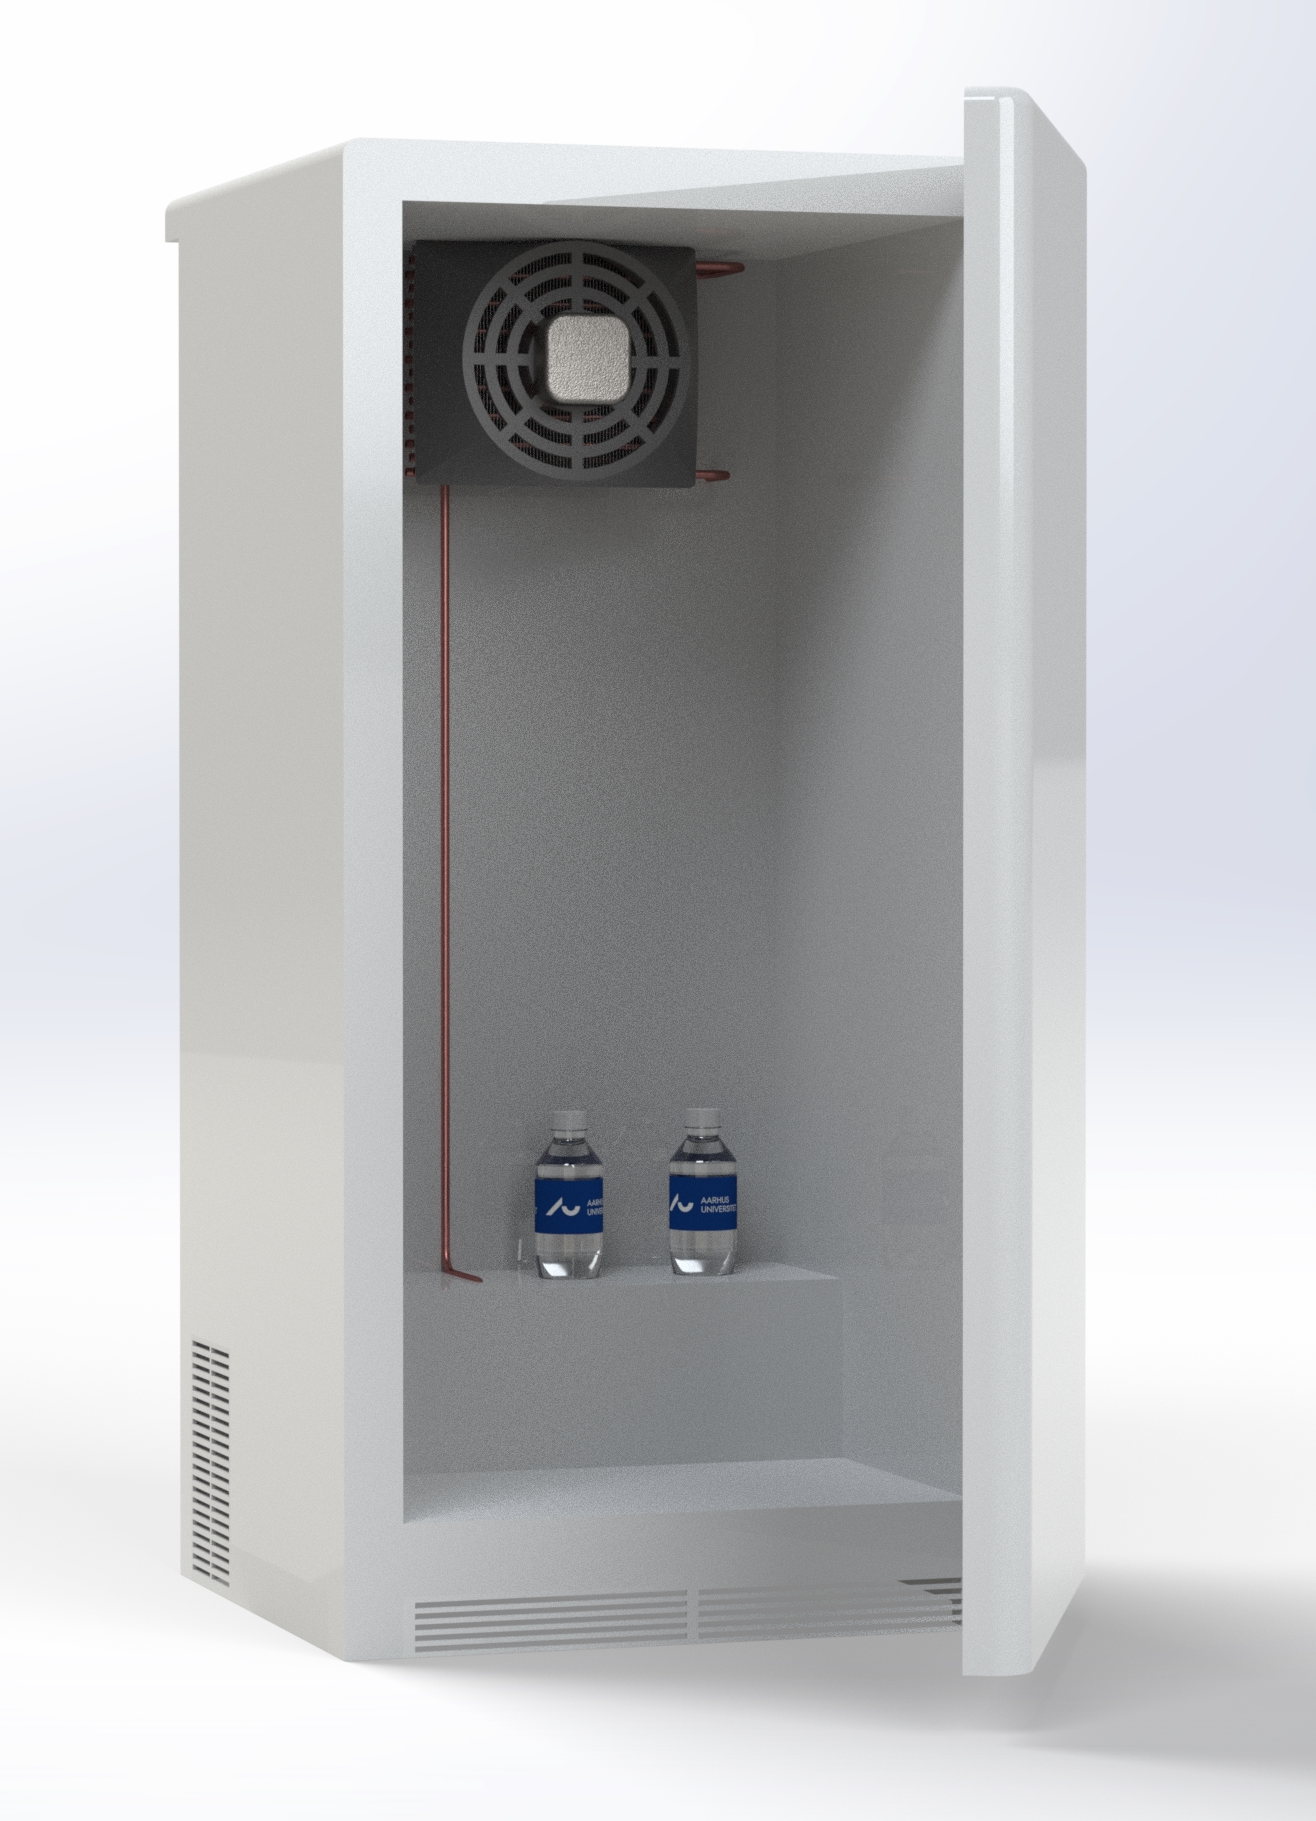
\includegraphics[width=0.8\textwidth]{Billeder/proto1}
    \caption{Senere prototype front}
    \label{fig:proto1}
\end{figure}

\section{Bud på viderebygget protype}
\label{sec:proto2}
\begin{figure}[H]
    \centering
    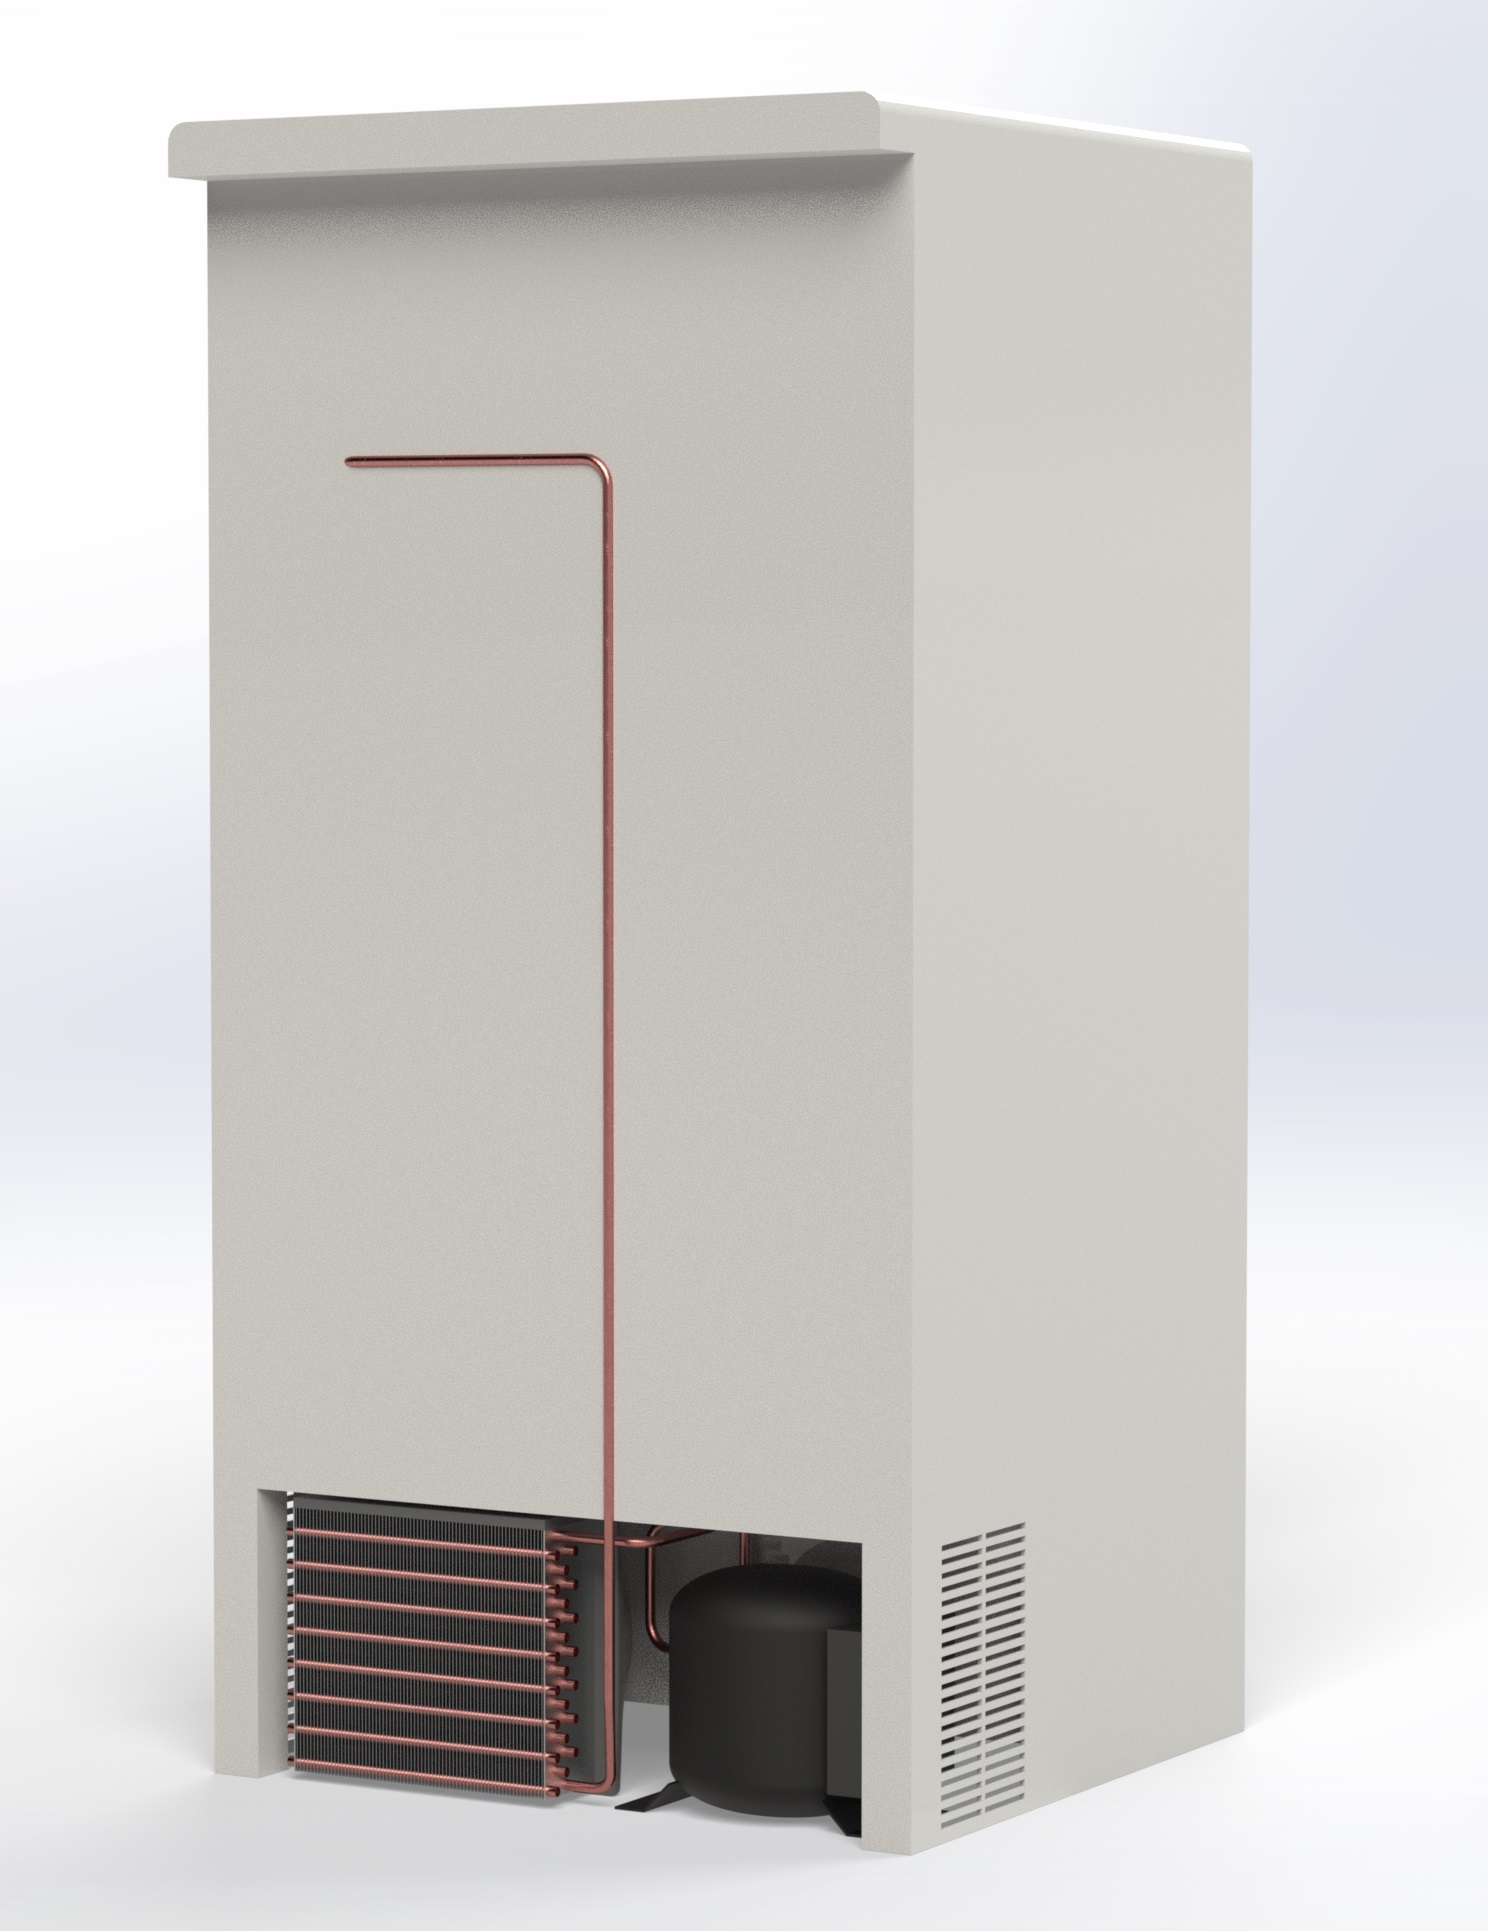
\includegraphics[width=1.0\textwidth]{Billeder/proto2}
    \caption{Senere prototype bag}
    \label{fig:proto2}
\end{figure}



\end{document}
